\documentclass{article}
%\documentclass[prl,amsmath,amssymb]{revtex4} % PRL

% margins of 1 inch:
\setlength{\topmargin}{-.5in}
\setlength{\textheight}{9in}
\setlength{\oddsidemargin}{0in}
\setlength{\textwidth}{6.5in}

\usepackage[pdftex]{hyperref} % hyperlink equation and bibliographic citations
\usepackage[dvips]{graphicx,color}
\usepackage{amsmath} % advanced math
\usepackage{verbatim}
\usepackage{natbib} % bibilography 
\usepackage{mciteplus} % collapse multiple citations in bibilography
\usepackage{multicol}
\usepackage[toc,page]{appendix} % http://tex.stackexchange.com/questions/49643/making-appendix-for-thesis


% from http://www.flakery.org/search/show/569
%\newcommand{\infint}{\ensuremath{\int_{-\infty}^{\infty}}}
\newcommand{\cf}{\textit{c.f.}} % "compare". In context the abbreviation advises readers to consult other material, drawing attention to related ideas that provide additional arguments or information.
\newcommand{\ie}{\textit{i.e.}} % i.e. is used to explain, clarify or rephrase a statement
\newcommand{\eg}{\textit{e.g.}} % “for the sake of example”. Used to introduce an example or list of examples to illustrate what is being discussed.
\newcommand{\eqn}[1]{Eq.\ (\ref{#1})}
\newcommand{\pfrac}[2]{\ensuremath{\frac{\partial #1}{\partial #2}}}
\newcommand{\pdg}{Physics Derivation Graph}

\begin{document}
\title{Introduction to the \pdg}

\author{Ben Payne$^{1}$\footnote{Corresponding author: ben.is.located@gmail.com}, Michael Goff$^{2}$\\
{\it $^{1}$Department of Fun, University Name \& Town, city, State Zip}\\
{\it $^{2}$Department of Mathematics, University of Maryland, Baltimore 21228}}

\date{\today}

\maketitle % declares end of title page
\begin{abstract}
An overview of the project. No prior background on this project is assumed. General knowledge of Physics and Mathematics at the first year college level is expected.
\end{abstract}


\begin{multicols}{2}

\tableofcontents

%\newpage

% Introduction: scope = ?

\section{Introduction\label{sec:intro}}

% relevant project background
The \pdg\ is an effort to capture mathematical physics knowledge. 

Historically, knowledge about physics has been recorded in the form of notes, letters, journal articles, and text books. 
The content is typically composed of text, equations, and pictures. 
The presentation is in a linear sequence, though references are often made to link the current section with previous sections and later sections. 

A recent addition to the toolset for capturing knowledge has been the use of linked webpages. 
A primary example of this is Wikipedia, an \href{https://en.wikipedia.org/wiki/HTML}{HTML}-based encyclopedia. 
Webpages such as Wikipedia still use text, equations, and pictures, but add a distinct capability: hyperlinks. 
Hypertext Markup Language offers the ability to connect content to any other content. 
This enables non-linear exploration of content, in contrast to a textbook which is designed to be read sequentially. 
The \pdg\ applies the concept of non-linear documentation to mathematical physics content. 

A \href{https://en.wikipedia.org/wiki/Graph_(mathematics)}{graph} is composed of nodes and edges. The graph associated with the \pdg\ has two essential types of nodes: mathematical expressions and inference rules. Every mathematical expression is connected to an inference rule by a directed edge. An example is provided here which illustrates the concepts.

\subsection{Example Derivation Step\label{sec:example}}
Derivations in Physics are composed of steps. 
Each step involves one or more expressions, and one inference rule. 
Inference rules are described in section~\ref{sec:inference_rules}. 

Frequency $f$ and period $T$ are related by
\begin{equation}
T\ f = 1
\label{eq:period_and_freq}
\end{equation}
Thus, frequency in terms of the period is
\begin{equation}
f = 1/T
\label{eq:freq_is_inverse_period}
\end{equation}
The relation between \eqn{eq:period_and_freq} and \eqn{eq:freq_is_inverse_period} is that both sides of \eqn{eq:period_and_freq} were divided by $T$. 

In the above example, there are two mathematical expressions: \eqn{eq:period_and_freq} and \eqn{eq:freq_is_inverse_period}. 
These expressions are related by an inference rule: ``Divide both sides of first expression by a scalar value to yield the second expression.'' 
This inference rule takes an argument, referred to here as the ``feed'', which in this example is $T$. 
This set of steps is shown graphically in~Fig.~\ref{fig:freq_period}

\begin{center}
\begin{figure}
%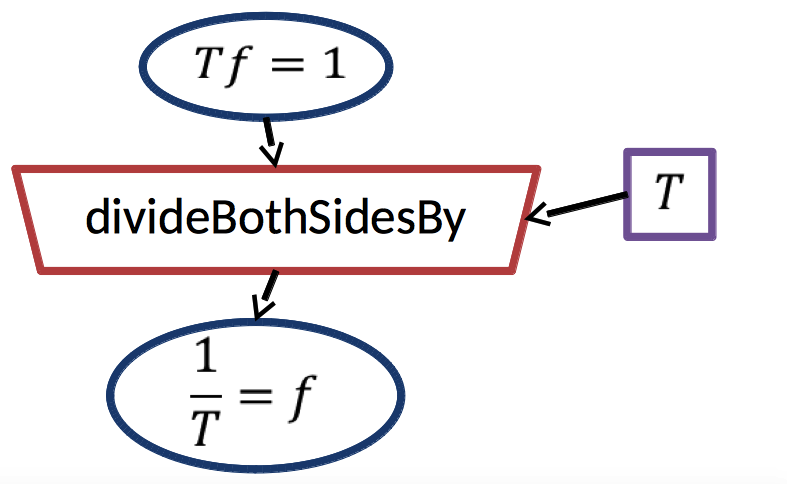
\includegraphics[scale=1]{images/frequency_period_relation.png}
\caption{Relation between period $T$ and frequency $f$.\label{fig:freq_period}}
\end{figure}
\end{center}

\section{Graph content\label{sec:content}}

The content associated with the \pdg\ takes the form of expressions (\textit{equations and inequalities}), symbols, and inference rules. \textit{An inference rule is an atomic transformation of one expression to another.} In the example provided in section~\ref{sec:example}, the two expressions are~\eqn{eq:period_and_freq} and~\eqn{eq:freq_is_inverse_period}. The symbols are period $T$ and frequency $f$. The inference rule being applied is ``Divide both sides of first equation by a value to yield the second equation.'' This inference rule takes an argument, referred to here as the ``feed'', which in this example is $T$. This simple step between two expressions is documented in five separate databases: expressions, symbols, feeds, inference rules, and connections. 

Each expression, symbol, and inference rule appears only once in the respective database. Each time an expression, symbol, or inference rule is used in a derivation, that unique instance is referenced. That referencing of unique nodes is what constructs the graph. For example, if \eqn{eq:period_and_freq} is used in two distinct derivations, the same expression is referenced. Similarly, when the symbol $T$ is used in any derivation, it refers to period. This referencing of unique expressions, symbols, and inference rules is done using a numeric identifier (alphanumeric for inference rules). This uniqueness of expressions, symbols, and inference rules is the core utility of the \pdg. This results in no duplication and fixed references (a static directed graph). The \pdg\ is designed to show one instance of each expression, but feeds and inference rules will have duplicates on the graph. 

Symbol re-use is common in science and can be addressed by the use of unique identifiers. For example, $c$ is typically used to stand for the speed of light, but the same symbol is also used in the quadratic equation
\begin{equation}
a x^2+b x+c =0.
\label{eq:quadratic}
\end{equation}
In this expression, we are not referring to the speed of light. This is distinguishable in the \pdg\ because the $c$ referring to the speed of light has a different numeric identifier than the $c$ in \eqn{eq:quadratic}. 

% inference rules
Inference rules are necessary to perform derivations in physics, but have received little attention as they are typically left to the field of logic. One result of an education in mathematics is building a library of inference rules, though that is not the common description in the field of math education. In Physics, knowing that it is valid to multiply both sides of an expression by one is assumed to have been learned in a math course. In the math course, the inference rule of multiplying both sides of an expression by one is taught with the common explanation that students need that inference rule to solve the relevant problems provided in the class. 
%These inference rules are a significant source of confusion and a source of error when used. Using inference rules correctly and applying them atomically are tasks which take patience and practice.
One of the consequences of constructing the \pdg\ is the enumeration of inference rules necessary for Physics. 

\section{Inference Rules\label{sec:inference_rules}}

Inference rules operate on expressions to produce new expressions. In section~\ref{sec:example}, the inference rule between \eqn{eq:period_and_freq} and \eqn{eq:freq_is_inverse_period} is ``Divide both sides of first expression by a scalar value to yield the second expression.''

Inference rules for the \pdg\ are designed to meet a threshold -- can the computer algebra system validate that the claim is true?

Inference rules are useful for catching simple mistakes by CAS validation. Common mistakes include not carrying the negative symbol through a derivation or unintentionally dropping a term. The inference rules are atomic (simplest step possible) and first order -- they only relate nearest-neighbor expressions.

\section{Administrivia}
General notes about the \pdg\ are provided here. 
\subsection{Scope of Project\label{sec:scope}}

The core of the \pdg\ is documenting the graph associated with mathematical physics. Once this content is available, there are many potential tasks. The following section (\ref{sec:stages}) provides a specific set of stages for potential future work. Not expected within the scope of the \pdg\ are inclusion of graphics, explanatory text, animations of concepts, and interactive models. 

Tasks in section~\ref{sec:stages} such as checking the validity of the graph using a Computer Algebra System, visualization of the graph, and interactivity of input are follow-on tasks once the graph content has been developed to describe mathematical physics.

\subsection{Access to Content\label{sec:access}}

The \pdg\ is free and open source under the Creative Commons Attribution-ShareAlike 3.0 Unported license. This content is free because it is intended to be accessible to anyone; cost should not be a barrier to access. The content is open source so that other researchers can build upon what exists. Once content is built, it should not need to be built again. 

\subsection{Similar Projects\label{sec:similar_projects}}

The scope and intention of the \pdg\ is unique, though aspects are shared by several active projects. Five examples are provided in this section: HyperPhysics, EquationMap, Formula Database, Symbolab, and Wolfram Alpha. The purpose is not to review these projects for utility or to comprehensively survey similar work. Instead, they are used here to contrast the scope and intention of the \pdg. 

The HyperPhysics website\cite{2015_Hyperphysics} is a static set of linked concept maps for topics in Physics. Concept maps are linked to text, graphs, and equations. The licensing of the content is described as ``not freeware or shareware'' by the author, though the site is free to access. Although hyperlinked concept maps are a departure from the standard textbook presentation of physics, the leaves of this tree are the same content found in textbooks. 

The website EquationMap\cite{2015_EquationMap} is an interface for derivations, focused primarily on mathematical sciences. There is no backend database of content; instead content is dynamically generated by the user. Equations are manually entered using \LaTeX syntax and the graph of the derivation can be visualized using the same interface. The content is not open source and access is currently free. This is close to what the GUI for the \pdg\ is intended to behave like, with the exception that EquationMap doesn't include the concept of atomic inference rules.


Formula Database\cite{2015_FormulaDatabase} is a website described by the authors as a ``math search engine'' which has a built-in equation editor. The search feature is not just matching the Latex input -- it understands dot product and cross product. They have created a browser-based equation editor, similar to the equation editor in Microsoft Word. The search is of a backend database of content. The backend database of equations and symbols was manually entered by the project authors. A team of people have been working since about 2010 on this project. The data is stored as a high-dimensional graph. This project is not open source but access is currently free. A commercial launch is planned, though no date has been publicized. 

The objective is to allow students to search through literature. If you are a researcher, you might want to find whether the model already exists in literature. The grand view is that formula-database will serve as a universal reference for equations.


SymboLab\cite{2015_Symbolab} is another backend database of content. This project is not open source but access is currently free. 

Wolfram Alpha\cite{2015_WolframAlpha} has a backend database of content which is not open source; access is a mix of free and paid. 

\section{Development Stages\label{sec:stages}}

This project is expected to evolve through distinct steps. Each step can be characterized by different users and associated requirements. 

% \subsection{Gathering Examples}
The first step is prototyping and involves a small number of expert users interested in gathering content for the \pdg. This exploratory phase involves research on appropriate syntax for the graph, brainstorming use cases, and minimal interaction with an external community. This is the current status of the project.

% \subsection{Proof of Concept}
The second phase is when sufficient examples exist to constitute a proof of concept. This requires breadth of coverage across all the domains of physics (\ie, classical mechanics, quantum mechanics, relativity, thermodynamics, statistical mechanics, etc). As a consequence, much of mathematics covered up to undergraduate level is likely to be required. 

% \subsection{Interface Creation}
Once the breadth of coverage is demonstrated, the next step is to enable development of in-depth creation for the \pdg. Currently, content is manually entered into an CSV database, and visualization of the graph is generated via the command line. To make both data entry and visualization more accessible to users and developers, a web browser-based interaction is planned. As noted in section~\ref{sec:scope}, this is outside of the project scope regarding graph content, but would make addition of content more accessible. Graph visualization libraries which are free and opensource are available, making this issue tractable. New standards such as HTML5 and libraries like d3js will be investigated to determine suitability. 

% \subsection{Community Utilization}
Adoption and utilization by the scientific and education communities is the intended outcome. Widespread use is dependent on having useful and reliable content, intuitive interfaces, and addressing a need. The \pdg\ does not currently exist, implying the needs being addressed are either unclear or sufficiently complex to make solution difficult. 

The steps listed above are intended to be worked on concurrently. Exploration of an intuitive interface can take place while examples are being gathered. In the next section, use cases which motivate users of this project are described. 



\section{Use Cases\label{sec:use_cases}}

While curiosity has driven the development of the \pdg, the resulting work is expected to be useful to multiple audiences and users. Viewers of the content could include students in math and physics, and analysis of the content could help shape curriculum. Contributors to the \pdg\ would be scientists who add new developments based on their work.

\subsection{Students in Math and Physics}

Currently students in Math and Physics are taught content using lectures, textbooks, and homework. The method of presentation varies, but the overarching story is often historically driven. Algebra is old, calculus is newer, and topology is recent. Classical mechanics is old, thermodynamics is newer, and quantum mechanics is recent. When teaching, these subjects are taught by building on previous content -- calculus leverages algebra, thermodynamics leverages classical mechanics. 

\subsection{Scientific Articles}

Peer-reviewed journal articles are one of the current methods of demonstrating value in the scientific community. Conciseness is a feature of this writing style, and the mathematics presented is correspondingly sparse -- just sufficient to covey the author's intention. This results in a burden on the reader of the article, either to take the author's claims on faith, or to rederive the mathematical expressions. A reader's derivation is complicated by implicit assumptions made by the author and unintentional mistakes in calculation. 

With journals allowing supplemental materials for articles, calculations could be included. However, it is not clear what the appropriate level of detail is in supplied calculations. The intention is to be able to reproduce the work, but 

validation via computer 

\subsection{Education Curriculum Design}

A less direct use case but potentially important impact of the \pdg\ is on understanding the relevance of what is being taught in the education system. Math classes essentially teach a set of inference rules, and physics is the application of those inference rules. The \pdg\ could answer two important questions: ``When am I going to use this inference rule?'' and ``What's the relative importance of this math skill?''

The focus for students in mathematics classes is on the technique, \ie, ``integrate both sides with respect to $Y$,'' and application is necessarily of secondary importance. Physics students are expected to know the mathematical techniques and teaching is focused on application. The \pdg\ can assist both scenarios. The student in a math class can see where the inference rules they learn are applied in Physics. The student in the Physics class can see which inference rules are required in their field. 

Each inference rule seems equally important, since it currently isn't known what the frequency of use for that inference rule is. From the \pdg, it is simple to count utilization of inference rules. Thus, we are able to measure the ratio of how often ``multiply both sides by X'' is used relative to ``integrate both sides with respect to $Y$.'' 

\section{Summary\label{sec:summary}}
This article provides an introduction to the \pdg. 

\section{Bibliography}

\bibliographystyle{unsrt}
\bibliography{../bibliography} % external bibtex flat-file database
\end{multicols}

\newpage
\appendix
%\begin{appendices}
%\section{Test cases in Latex and MathML}\label{sec:appendix_test_cases}

\subsection{Case 1: polynomial}

\begin{equation}
a x^2 + b x + c = 0
\label{eq:polynomial_case1}
\end{equation}
Latex: 
\begin{verbatim}
a x^2 + b x + c = 0
\end{verbatim}

SymPy:
\verbatiminput{sympy_case1_polynomial.py}

Presentation MathML:
% http://www.mathmlcentral.com/Tools/FromMathML.jsp

%\begin{figure}
%\begin{center}
%\includegraphics[scale=1,bb=0 0 111 19]{images/case1_polynomial_mathML_presentation.gif}
%\caption{Case 1 polynomial in Presentation MathML}
%\end{center}
%\end{figure}

\verbatiminput{mathML_presentation_case1_polynomial.xml}

Content MathML:
\verbatiminput{mathML_content_case1_polynomial.xml}

\subsection{Case 2: Stoke's theorem}
\begin{equation}
\int \int_{\sum} \vec{\nabla} \times \vec{F} \dot d\sum = \oint_{\partial \sum} \vec{F}\dot d\vec{r}
\label{eq:stokes_case2}
\end{equation}
Latex:
\begin{verbatim}
\int \int_{\sum} \vec{\nabla} \times \vec{F} \dot d\sum = 
\oint_{\partial \sum} \vec{F}\dot d\vec{r}
\end{verbatim}

SymPy:
\verbatiminput{sympy_case2_stokes.py}


Presentation MathML:
\verbatiminput{mathML_presentation_case2_stokes.xml}

Content MathML:
\begin{verbatim}
<math xmlns="http://www.w3.org/1998/Math/MathML">

</math>
\end{verbatim}

\subsection{Case 3: Tensor analysis}
\begin{equation}
Y^i(X_j) = \delta^i_{\ j}
\label{eq:tensor_analysis_case3}
\end{equation}
Latex: 
\begin{verbatim}
Y^i(X_j) = \delta^i_{\ j}
\end{verbatim}

SymPy:
\verbatiminput{sympy_case3_tensor.py}


Presentation MathML:
\verbatiminput{mathML_presentation_case3_tensor.xml}

Content MathML:
\begin{verbatim}
<math xmlns="http://www.w3.org/1998/Math/MathML">

</math>
\end{verbatim}


\subsection{Case 4a: creation operator}
\begin{equation}
\hat{a}^+ |n\rangle = \sqrt{n+1} |n+1\rangle
\label{eq:creation_operator_case4a}
\end{equation}

\begin{verbatim}
\hat{a}^+ |n\rangle = \sqrt{n+1} |n+1\rangle
\end{verbatim}

SymPy:
\verbatiminput{sympy_case4a_creation.py}


Presentation MathML:
\verbatiminput{mathML_presentation_case4a_creation.xml}

Content MathML:
\begin{verbatim}
<math xmlns="http://www.w3.org/1998/Math/MathML">

</math>
\end{verbatim}

\subsection{Case 4b: uncertainty principle}
\begin{equation}
\sigma_x \sigma_p \geq \frac{\hbar}{2}
\label{eq:uncertainty_principle_case4b}
\end{equation}

\begin{verbatim}
\sigma_x \sigma_p \geq \frac{\hbar}{2}
\end{verbatim}

SymPy:
\verbatiminput{sympy_case4b_uncertainty.py}


Presentation MathML:
\verbatiminput{mathML_presentation_case4b_uncertainty.xml}

Content MathML:
\begin{verbatim}
<math xmlns="http://www.w3.org/1998/Math/MathML">

</math>
\end{verbatim}

\subsection{Case 4c: L\"{u}ders projection}
\begin{equation}
 |\psi\rangle \rightarrow \sum_n  |c_n|^2 P_n,\ \rm{where}\ P_n = 
 \sum_i |\psi_{ni}\rangle \langle \psi_{ni}|
\label{eq:Luders_projection_case4c}
\end{equation}

\begin{verbatim}
 |\psi\rangle \rightarrow \sum_n  |c_n|^2 P_n,\ \rm{where}\ P_n = \sum_i |\psi_{ni}\rangle \langle \psi_{ni}|
\end{verbatim}

SymPy:
\verbatiminput{sympy_case4c_projection.py}


Presentation MathML:
\begin{verbatim}
<math xmlns="http://www.w3.org/1998/Math/MathML">

</math>
\end{verbatim}

Content MathML:
\begin{verbatim}
<math xmlns="http://www.w3.org/1998/Math/MathML">

</math>
\end{verbatim}

%\end{appendices}


\end{document}
